\chapter{D\'eveloppement du module d'extension <<qtype\_essayhelper>>}
\GT{Tu parles des fonctionnalit\'es, et des tests, mais tu ne parles
pas vraiment de ce que tu as fait --- c'est comme si tu d\'ecrivais le
<<quoi>> (fonctionnalit\'es et tests, les tests pouvant aussi \^etre
vus comme des exemples d'utilisation, donc le <<quoi>>, mais tu ne
d\'ecris le <<comment>> --- conception et mise en oeuvre (sauf pour
les d\'etails de la racination.  En d'autres mots, je trouve
qu'apr\`es lecture de ce chapitre, on ne comprend pas exactement
comment ton module est structur\'e, comment il s'ins\`ere dans
l'architecture.  Peut-\^etre le chapitre sur Moodle devrait discuter
un peu plus --- peut-\^etre avec un graphique/diagramme --- de cette
architecture modulaire.  Ensuite, ici, tu pourrais pr\'esenter de
fa\c{c}on un peu plus sp\'ecifique la structure, l'organisation du
code que tu as d\'evelopp\'e.  Parce que ce n'est pas clair je trouve.
On voit mal l'envergure, le style d'organisation du code, etc.}
\PG{J'ai ajout\'e une section architecture plus bas afin d'aider \`a comprendre un peu plus le <<Comment>>}
Le site de Moodle donne une br\`eve introduction \`a la cr\'eation d'un nouveau type de question \footnote{\url{https://docs.moodle.org/dev/Question\_types\#Question\_type\_plug\_in\_development}}.
Un gabarit est disponible afin d'aider \`a d\'ebuter, mais le site conseille de modifier ou copier un type de question existant s'il est similaire au type de question que nous voulons d\'evelopper.
Dans notre cas, nous allons utiliser le type de question \og qtype\_essay \fg{} comme base, car il poss\`ede presque toutes les fonctionnalit\'es d\'esir\'ees.
Les commentaires de \emph{copyrights} ont \'et\'e ajust\'es comme illustr\'e \`a l'exemple de code~\ref{code:commentaire}.
\begin{lstfloat}
\begin{lstlisting}[frame=l]
/**
 * Essay for correction helper question definition class.
 *
 * @package    qtype
 * @subpackage essayhelper
 * @copyright  2018 Philippe Girard
 * @license    http://www.gnu.org/copyleft/gpl.html GNU GPL v3 or later
 *
 * Inspired by:
 * @package    qtype
 * @subpackage essay
 * @copyright  2009 The Open University
 * @license    http://www.gnu.org/copyleft/gpl.html GNU GPL v3 or later
 */
\end{lstlisting}
\caption{Exemple des commentaires dans les fichiers du module d'extension.}
\label{code:commentaire}
\end{lstfloat}
\section{Fonctionnalit\'es de qtype\_essayhelper}
Plusieurs fonctionnalit\'es du module d'extension \og qtype\_essay \fg{} ont \'et\'e enlev\'ees:
\begin{description}
  \item[\'editeur de texte WYSIWIG]
  
  Cet \'editeur permet de modifier facilement l'apparence du texte.
  Ceci permet, entre autres, de surligner, de souligner, de mettre en gras, de mettre en italique et plus encore.
  Comme on ne peut pas enlever des options WYSIWIG pour un seul module d'extension, cela devient complexe de trouver une mise en forme qui permet de mettre en \'evidence les mots cl\'es, car un \'etudiant pourrait, par erreur, reproduire la m\^eme mise en forme.
  
  \item[Remise de fichier]
  
  Il est possible d'\'ecrire directement dans la zone de texte ou de remettre un document texte (configurable par l'enseignant).
  Comme le module d'extension n'aidera pas \`a corriger les textes remis par fichier, cette option a \'et\'e enlev\'ee.
\end{description}
Plusieurs fonctionnalit\'es sont rest\'ees dans le nouveau module d'extension:
\begin{description}
  \item[R\'etroaction g\'en\'erale]
  
  Cette fonctionnalit\'e permet de laisser un commentaire \`a l'\'etudiant une fois que la correction est termin\'ee.
  Par exemple, l'enseignant pourrait laisser des explications sur les erreurs courantes.
  
  \item[Mod\`ele de r\'eponse]
  
  Ceci permet de pr\'eremplir la zone de texte de l'\'etudiant avec le texte donn\'e.
  Par exemple, un en-t\^ete de fonction pour une question de programmation ou la liste des mots \`a d\'efinir.
  
  \item[Information de l'\'evaluateur]
  
  Ceci affiche un texte pour le correcteur seulement.
  Utile pour voir facilement le bar\`eme de correction ou donner des instructions au correcteur.
  Est affich\'e sous la r\'eponse de l'\'etudiant lors de la correction.
\end{description}
Finalement, les fonctionnalit\'es suivantes ont \'et\'e ajout\'ees:
\begin{description}
  \item[Mots-cl\'es]
  
  Les mots-cl\'es sont mis en \'evidence dans la r\'eponse de l'\'etudiant lors de la correction manuelle.
  \item[R\'eponse officielle de l'enseignant]
  
  Affiche ce texte \`a droite de la r\'eponse de l'\'etudiant lors de la correction.
  Les mots-cl\'es sont mis en \'evidence aussi dans ce texte.
\end{description}
\section{Architecture de qtype\_essayhelper}
L'installation d'un module d'extension dans Moodle est tr\`es simple.
Premi\`erement il faut mettre le r\'epertoire du module d'extension au bon endroit.
Par exemple, un type de question doit se trouver dans le dossier \og question/type \fg{}.
Deuxi\`emement il faut se connecter sur Moodle en tant qu'administrateur.
Moodle d\'etectera automatiquement qu'il y a un nouveau module d'extension.
Finalement, Moodle proposera \`a l'administrateur d'installer le nouveau module d'extension avant que l'administrateur puisse acc\'eder au syst\`eme.
\`A l'int\'erieur du r\'epertoire du module d'extension, les fichiers doivent avoir le bon nom et \^etre au bon endroit.
L'architecture est illustr\'ee \`a la figure \ref{dev-architecture} et d\'ecrite ci-dessous.
\begin{figure}[h!]
  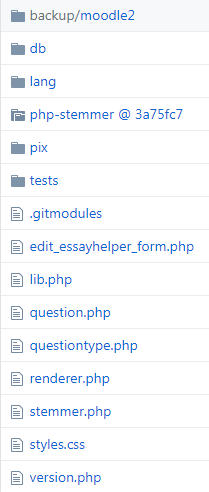
\includegraphics[scale=0.7]{images/architecture.png}
  \caption{Processus de racination Snowball pour la langue fran\c{c}aise.}
  \label{dev-architecture}
\end{figure}
\begin{description}
 \item[backup/moodle2]
 
 Fichier qui g\`ere la sauvegarde et la restauration des questions de ce type.
 Le sous-dossier moodle2 indique que cette fonctionnalit\'e existe seulement pour la version 2 de Moodle et les suivantes.
 
 \item[db]
 
 Contiens un fichier \og install.xml \fg{} qui d\'efinit la table de base de donn\'ees \`a cr\'eer pour ce module d'extension.
 
 \item[lang]
 
 Contient un sous-dossier par langue support\'ee sois \og fr \fg{} et \og en \fg{} dans ce projet.
 Chaque sous-dossier contient un fichier PHP qui d\'efini les cha\^ines de traductions.
 Ce dossier de traduction est valide pour les fonctionnalit\'es Moodle, pas pour la racination.
 
 \item[php-stemmer]
 
 Sous-module git pour ce projet uniquement.
 Pointe vers la librairie de racination utilis\'e et d\'ecrit au chapitre \ref{chap:phpstemmer}.
 
 \item[pix]
 
 Contiens l'ic\^one du type de question.
 Cette ic\^one est uniquement visible lorsque l'enseignant choisit le type de question pour une nouvelle question.
 
 \item[tests]
 
 Ce dossier contient tous les tests unitaires et d'acception du module d'extension.
 Pour plus de d\'etail, voir la section \ref{dev_test}.
 
 \item[edit\_essayhelper\_form.php]
 
 D\'efini le formulaire que l'enseignant remplis lorsqu'il cr\'e une question de ce type.
 Il faut uniquement d\'efinir les champs sp\'ecifiques au type de question actuel, Moodle ajoute ajoute automatiquement les champs de base comme le nom de la question et la valeur en point de la question dans le questionnaire.
 
 \item[question.php]
 
 G\`ere la r\'eponse \`a une question.
 D\'efini le comportement de question \`a utiliser, comment afficher la r\'eponse (appel renderer.php) et valide la pr\'esence d'une r\'eponse.
 
 \item[questiontype.php]
 
 G\`ere la cr\'eation, modification et suppression d'une question de ce type.
 
 \item[renderer.php]
 
 G\`ere l'affichage d'une question et des r\'eponses.
 Permets de contr\^oler la zone de texte pour une nouvelle r\'eponse ou pour la modifier.
 Permets aussi de changer l'affichage de la r\'eponse pour le correcteur.
 C'est dans ce fichier que nous allons surtout travailler.
 
 \item[stemmer.php]
 
 Fichier sp\'ecialement con\c{c}u pour ce module d'extension.
 C'est dans ce fichier que nous g\'erons le lien entre Moodle et \texttt{php-stemmer}.
 
 \item[styles.css]
 
 Fichier css pour notre module d'extension.
 
 \item[version.php]
 
 Fichier contenant 4 informations:
 \begin{itemize}
   \item \og component \fg{}
   
   Nom du module d'extension qui sera utilis\'e dans la base de donn\'ees Moodle.
   Dans ce projet il s'agit de \og qtype\_essayhelper \fg{}.
   
   \item \og version \fg{}
   
   Num\'ero de version du module d'extension dans le format \og aaaammjj00 \fg{} utilisant la date.
   Les deux derniers \og 0 \fg{} sont utilis\'es pour faire plus qu'une version par jour.
   Pour que Moodle prenne en compte les changements au fichier \og install.xml \fg{} (pour la base de donn\'ees), il faut changer le num\'ero de version.
   
   \item \og requires \fg{}
   
   Num\'ero de version Moodle n\'ecessaire au bon fonctionnement du module d'extension utilisant aussi le format \og aaaammjj00 \fg{}.
   Notre module d'extension utilise la m\^eme d\'ependance que \og qtype\_essay \fg{} soit \og 2015111600 \fg{} qui repr\'esente Moodle 3.0.
   
   \item \og maturity \fg{}
   
   La maturit\'e du module d'extension.
   Notre module d'extension se trouve encore en \textit{MATURITY\_ALPHA}.
 \end{itemize}
\end{description}
Dans tous les fichiers il y a eu un peu d'adaptation du code afin de passer de \og qtype\_essay \fg{} \`a \og qtype\_essayhelper \fg{}.
\section{Code Moodle de qtype\_essayhelper}
Le code du module d'extension est peu complexe.
Ce qui cause de la complexit\'e dans le projet r\'eside dans l'interaction entre le coeur de Moodle et ces classes.
La figure \ref{dev-class} illustre les diff\'erentes classes qui seront d\'etaill\'ees dans les prochaines pages.
\begin{figure}[h!]
  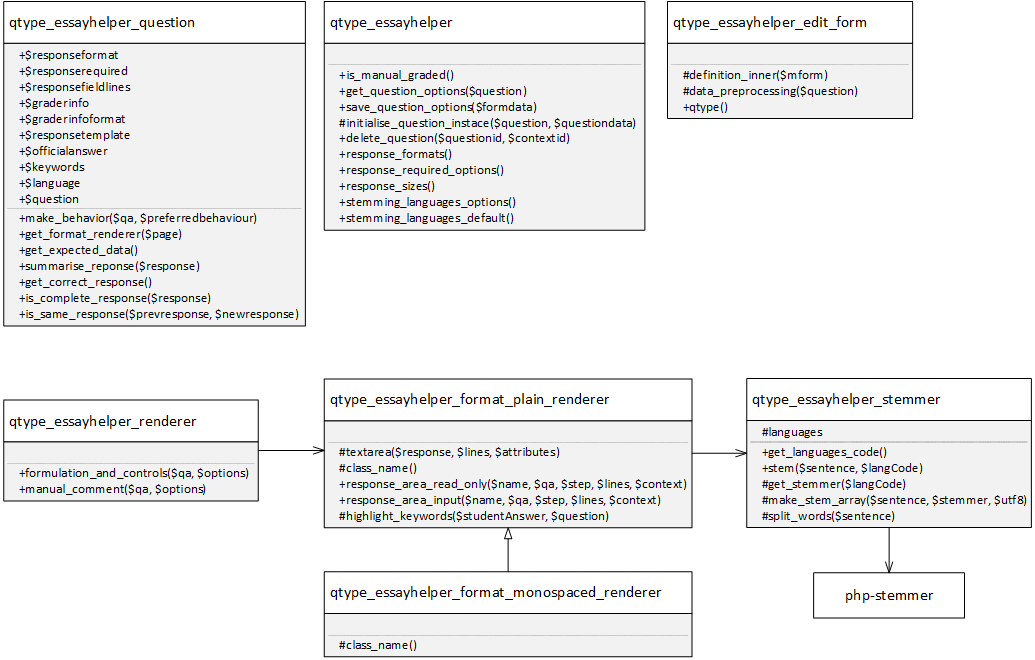
\includegraphics[scale=0.5]{images/class.png}
  \caption{Principales classes de \texttt{qtype\_essayhelper}.}
  \label{dev-class}
\end{figure}
\subsection*{Classe \texttt{qtype\_essayhelper\_edit\_form}}
Cette classe g\`ere le formulaire de cr\'eation et modification de question pour ce type de question.
Elle poss\`ede deux fonctions, la premi\`ere est \og definition\_inner \fg{} qui permet d'ajouter des champs au formulaire de base de cr\'eation de questions.
Le formulaire de base comporte quelques champs tels que le titre de la question, le texte de la question ainsi que le nombre de points que vaut cette question.
La gestion des champs de base se fait automatiquement par Moodle, il ne reste donc qu'\`a ajouter nos champs suppl\'ementaires pour notre type de question.
L'ajout de champs se fait avec un objet formulaire fourni par Moodle.
L'exemple de code \ref{code:formdefinition} illustre l'ajout des champs d'aide \`a la correction dans le formulaire de notre module d'extension.
La fonction principale de cet objet est addElement qui prend 4 param\`etres:
\begin{enumerate}
  \item Le type d'\'el\'ement;
  \item Le nom du champ doit \^etre le m\^eme que dans la base de donn\'ees;
  \item Le texte \`a afficher, la fonction \textit{get\_string} traduit la cha\^ine donn\'ee en premier param\`etre dans les fichiers de traductions du module d'extension donn\'e dans le deuxi\`eme param\`etre;
  \item Optionnellement, des options suppl\'ementaires.
\end{enumerate}
\begin{lstfloat}
\begin{lstlisting}[frame=l]
$qtype = question_bank::get_qtype('essayhelper');
$mform->addElement('header', 'essayhelper', get_string('essayhelperheader', 'qtype_essayhelper'));
$mform->setExpanded('essayhelper');
$mform->addElement('textarea', 'officialanswer', get_string('officialanswer', 'qtype_essayhelper'),
 array('rows' => 10, 'cols' => 100));
$mform->addElement('textarea', 'keywords', get_string('keywords', 'qtype_essayhelper'),
 array('rows' => 10, 'cols' => 60));
$mform->addHelpButton('keywords', 'keywords', 'qtype_essayhelper');
\end{lstlisting}
\caption{Extrait du code de la fonction definition\_inner de la classe qtype\_essayhelper\_edit\_form.}
\label{code:formdefinition}
\end{lstfloat}
La deuxi\`eme fonction de cette classe permet de sauvegarder les champs du formulaire.
Tous les champs non reconnus par Moodle doivent \^etre trait\'es manuellement dans cette fonction comme illustr\'ee \`a l'exemple de code \ref{code:formpreprocessing}.
\begin{lstfloat}
\begin{lstlisting}[frame=l]
$question->responsetemplate = $question->options->responsetemplate;
$question->officialanswer = $question->options->officialanswer;
$question->keywords = $question->options->keywords;
\end{lstlisting}
\caption{Extrait du code de la fonction data\_preprocessing de la classe qtype\_essayhelper\_edit\_form.}
\label{code:formpreprocessing}
\end{lstfloat}
\subsection*{Classe \texttt{qtype\_essayhelper\_question}}
Cette classe g\`ere la r\'eponse \`a une question, que ce soit pour une nouvelle r\'eponse, une modification de r\'eponse ou afficher la r\'eponse au correcteur.
Les fonctions d\'efinies dans cette classe sont:
\begin{description}
  \item[make\_behaviour] Retourne le comportement utilis\'e par le type de question. \texttt{manualgraded} dans ce cas.
  \item[get\_format\_renderer] Retourne la classe \texttt{qtype\_essayhelper\_renderer} qui s'occupera de l'affichage de la question.
  \item[get\_expected\_data] Retourne ce que la r\'eponse de l'\'etudiant doit contenir. Dans notre cas il y a seulement une r\'eponse textuelle.
  \item[summarise\_response] Retourne un r\'esum\'e de la r\'eponse de l'\'etudiant, dans notre cas il s'agit de la r\'eponse directement. Sera utilis\'e dans les modules de corrections afin de donner un aper\c{c}u de la r\'eponse de chaque \'etudiant.
  \item[get\_correct\_response] Devrait retourner la bonne r\'eponse \`a la question. Notre fonction retourne null afin d'indiquer \`a Moodle qu'il n'y a pas de bonne r\'eponse.
  \item[is\_complete\_response] V\'erifie si l'\'etudiant a r\'epondu \`a la question. Nous v\'erifions simplement s'il y a une r\'eponse non-vide.
  \item[is\_same\_response] D\'etermine si l'\'etudiant a modifi\'e sa r\'eponse.
\end{description}
\subsection*{Classe qtype\_essayhelper}
Cette classe g\`ere les options du type de question ainsi que les interactions \`a la base de donn\'ees.
Les fonctions d'interactions avec la base de donn\'ees:
\begin{description}
  \item[is\_manual\_graded] Retourne \texttt{vrai} dans notre cas pour indiquer que la question doit se corriger manuellement.
  \item[get\_question\_options] R\'ecup\`ere les options pour la question d\'efinie dans la base de donn\'ees. Nous retournons simplement le r\'esultat de la requ\^ete.
  \item[save\_question\_options] Ici il faut prendre les donn\'ees du formulaire et les ajout\'er dans la base de donn\'ees. G\`ere la cr\'eation et la modification de la question.
  \item[initialise\_question\_instance] Initialise l'instance de la question en ajoutant les options \`a l'objet repr\'esentant la question.
  \item[delete\_question] Supprime la question de la base de donn\'ees. Notre type de question n'utilise qu'une seule table, il s'agit donc d'une seule requ\^ete \texttt{DELETE}.
\end{description}
Les options du type de question sont des listes d\'eroulantes dans le formulaire de cr\'eation et modification de question.
Les fonctions qui d\'efinissent les options sont:
\begin{description}
  \item[response\_formats] Retourne les formats de r\'eponses possibles soit \og Texte pur \fg{} et \og Texte pur, police monospace \fg{} .
  \item[response\_required\_options] Retourne deux options soit \og Requiers la saisie d'un texte par le participant \fg{} et \og Saisie de texte optionnelle \fg{}.
  \item[response\_sizes] Donne le nombre de lignes par d\'efaut que contiendra le champ de r\'eponse. Nous donnons les options de 5 \`a 40 avec des intervalles de 5.
  \item[stemming\_languages\_options] R\'ecup\`ere toutes les langues disponibles pour la racination et les traduits dans la langue de l'utilisateur avec la fonction \texttt{PHP Locale::getDisplayName}.
  \item[stemming\_languages\_default] Trouve la langue de racination par d\'efaut en se basant sur la langue actuelle de l'utilisateur. Si la langue n'est pas reconnue, nous utilisons l'anglais.
\end{description}
\subsection*{Classe qtype\_essayhelper\_renderer}
Cette classe g\`ere l'affichage de la question aux \'etudiants lorsqu'ils r\'epondent ainsi que l'affiche de la r\'eponse de l'\'etudiant lors de la relecture de celui-ci ou lors de la correction.
Elle ne contient que deux fonctions:
\begin{description}
  \item[formulation\_and\_controls] G\`ere l'affichage du texte de la question, la zone de r\'eponse de l'\'etudiant est g\'er\'ee par la classe \texttt{ qtype\_essayhelper\_format\_plain\_renderer}.
  \item[manual\_comment] G\`ere l'affichage de la zone de commentaire de l'enseignant lors de la correction. Pour chaque r\'eponse l'enseignant peut laisser un commentaire.
\end{description}
\subsection*{qtype\_essayhelper\_format\_plain\_renderer}
Cette classe g\`ere la r\'eponse de l'\'etudiant.
\begin{description}
  \item[textarea] Fonction prot\'eg\'ee qui construit la zone de texte lorsqu'un \'etudiant r\'epond \`a la question.
  \item[class\_name] Fonction prot\'eg\'ee qui retourne le nom de la classe css \`a appliquer sur la balise \texttt{HTML} englobant la question et la r\'eponse.
  \item[response\_area\_read\_only] Fonction qui affiche le texte de la r\'eponse pour consultation seulement. Si c'est un enseignant ou un correcteur qui consulte la question dans le module de correction manuel on affiche la r\'eponse de l'enseignant \`a c\^ot\'e de la r\'eponse de l'\'etudiant et on met en \'evidence les mots clés
  \item[response\_area\_input] Affiche la zone de texte cr\'e\'e par la fonction \texttt{textarea} afin que l'\'etudiant puisse r\'epondre \`a la question.
  \item[highlight\_keywords] Met en \'evidence les mots-cl\'es trouv\'es dans le texte par la racination.
\end{description}
La classe \texttt{qtype\_essayhelper\_format\_monospaced\_renderer} hérite de la classe \texttt{qtype\_essayhelper\_format\_plain\_renderer} et red\'efini seulement la fonction \texttt{class\_name}.
Le CSS correspondant \`a la classe retourn\'ee est d\'efini dans le module d'extension \texttt{qtype\_essay}.
Un exemple de l'interaction de toutes ces classes avec Moodle est illustr\'e \`a la figure \ref{dev-diagramme}.
Cet exemple illustre l'ouverture d'un questionnaire par un \'etudiant.
\begin{landscape}
\begin{figure}[h!]
  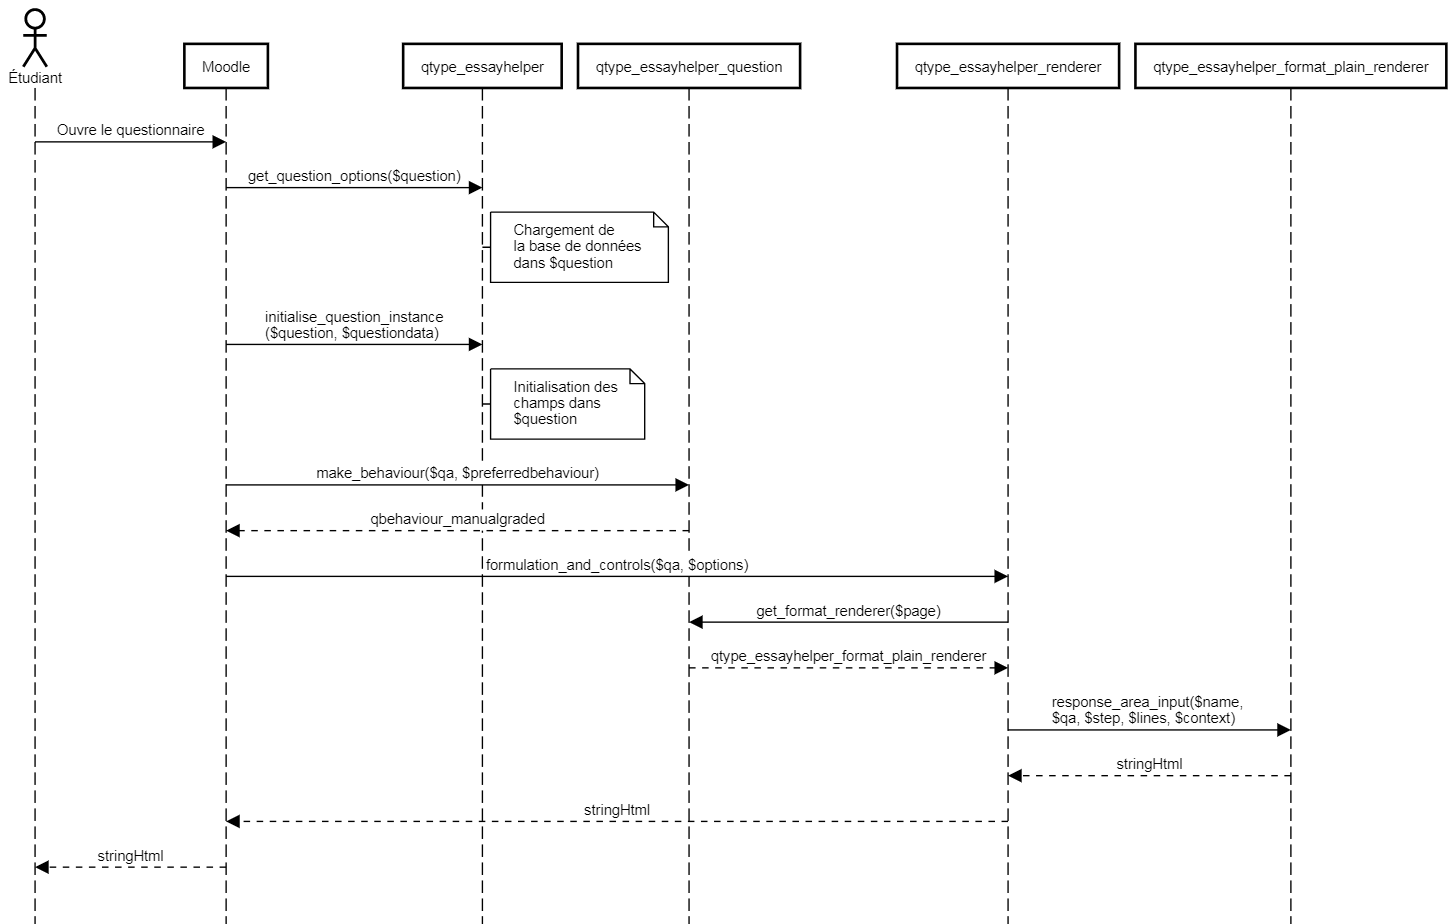
\includegraphics[scale=0.4]{images/diagramme-flux.png}
  \caption{Interaction entre Moodle et le module d'extension \texttt{qtype\_essayhelper}.}
  \label{dev-diagramme}
\end{figure}
\end{landscape}
\section{D\'etection des mots cl\'es}
Comme cit\'e dans le \autoref{chap:keywords}, nous utilisons la biblioth\`eque \texttt{php-stemmer} afin de trouver la racine de chaque mot.
Pour trouver la racine de tous les mots du texte, il faut d\'ebuter par les isoler.
Les caract\`eres non alphanum\'eriques sont remplac\'es par des espaces et le texte est d\'ecoup\'e par des caract\`eres d'espacement (espace, saut de ligne, tabulation, etc.) tel qu'illustr\'e dans l'extrait de code \ref{code:isoler}.
\begin{lstfloat}
\begin{lstlisting}[frame=l]
$words = preg_split('/(\s|\')/', preg_replace('/[^[:alnum:][:space:]]/u', ' ', $sentence));
\end{lstlisting}
\caption{Isoler les mots du texte.}
\label{code:isoler}
\end{lstfloat}
Ensuite, chaque mot est associ\'e avec sa racine trouv\'ee avec l'algorithme Snowball tel qu'illustr\'e dans l'extrait de code \ref{code:racinationsnowball}.
Chaque mot-cl\'e a, pr\'ealablement, aussi \'et\'e r\'eduit \`a sa racine avec l'algorithme Snowball.
\begin{lstfloat}
\begin{lstlisting}[frame=l]
foreach ($words as $word) {
 if ($word) {
  if (Wamania\Snowball\Utf8::check($word)) {
   $stem = $stemmer->stem($word);
   if (isset($stems[$stem])) {
    if (!in_array($word, $stems[$stem])) {
     $stems[$stem][] = $word;
    }
   } else {
    $stems[$stem] = array($word);
   }
  } else {
   $stems[] = $word;
  }
 }
}
\end{lstlisting}
\caption{Racination des mots avec Snowball.}
\label{code:racinationsnowball}
\end{lstfloat}
Finalement les mots-cl\'es trouv\'es dans le texte sont mis en \'evidence.
\begin{lstfloat}
\begin{lstlisting}[frame=l]
$usedKeywords = array_intersect(array_keys($stems), $keywords);
foreach ($usedKeywords as $keyword) {
 $words = $answerWords[$keyword];
 foreach ($words as $word) {
  $studentAnswer = str_replace($word, '<b><u>' . $word . '</u></b>', $studentAnswer);
 }
}
\end{lstlisting}
\caption{Mise en \'evidence des mots-cl\'es trouv\'es.}
\label{code:mots-cles}
\end{lstfloat}
\section{Tests} \label{dev_test}
Les tests du module d'extension \og qtype\_essay \fg{} ont \'et\'e conserv\'es et adapt\'es \`a ce nouveau module d'extension.
Le fonctionnement de base d'un module d'extension (cr\'eation de question, modification de question, r\'epondre \`a la question, etc.) a donc facilement \'et\'e test\'e.
Il ne restait plus qu'\`a tester les nouvelles fonctionnalit\'es de mots-cl\'es et d'affichage de la r\'eponse de l'enseignant.
\subsection{Tests d'acceptation} \label{dev_test_acceptation}
Les tests d'acceptation r\'ecup\'er\'es du module d'extension \textit{qtype\_essay} ont permis de trouver quelques probl\`emes  dans le nouveau module d'extension.
Par exemple, la fonctionnalit\'e \textit{Backup and restore} ne fonctionnait pas pour les questions avec le nouveau type de question \textit{qtype\_essayhelper}.
Le probl\`eme venait d'un dossier manquant dans le nouveau module d'extension.
Le dossier \textit{backup} dans le module d'extension \textit{qtype\_essayhelper} ne contiens pas des copies de sauvegardes du module d'extension, mais plusieurs versions de la fonctionnalit\'e \textit{Backup and restore}.
\subsection{Tests unitaires} \label{dev_test_unitaire}
La biblioth\`eque de racination \texttt{php-stemmer} est d\'ej\`a test\'e unitairement et valid\'e \`a l'aide d'un dictionnaire qui associe les mots \`a leurs racines.
Il ne restait donc qu'\`a tester l'int\'egration entre Moodle et la biblioth\`eque de racination.
